\documentclass[compress]{beamer}
%--------------------------------------------------------------------------
% Common packages
%--------------------------------------------------------------------------
\usepackage[T1]{fontenc}
\usepackage{graphicx}
\usepackage{multicol}
\usepackage{tabularx,ragged2e}
\usepackage{booktabs}
\usepackage{listings}
\lstset{ %
language=erlang,
basicstyle=\normalsize\ttfamily,
keywordstyle=,
numbers=left,
numberstyle=\tiny\ttfamily,
stepnumber=1,
showspaces=false,
showstringspaces=false,
showtabs=false,
breaklines=true,
frame=tb,
framerule=0.5pt,
tabsize=4,
framexleftmargin=0.5em,
framexrightmargin=0.5em,
xleftmargin=0.5em,
xrightmargin=0.5em
}

%--------------------------------------------------------------------------
% Load theme
%--------------------------------------------------------------------------
\usetheme{hsrm}

\usepackage{tikz}
\usetikzlibrary{mindmap,backgrounds}

%--------------------------------------------------------------------------
% General presentation settings
%--------------------------------------------------------------------------
\title{Functional Algebra by Example}
\date{Last Updated: \today}
\author{Susan Potter \small{@SusanPotter}}

%--------------------------------------------------------------------------
% Notes settings
%--------------------------------------------------------------------------
%\setbeameroption{show notes}

\begin{document}
%--------------------------------------------------------------------------
% Titlepage
%--------------------------------------------------------------------------
\begin{frame}{Functional Algebra By Example}
  \begin{figure}
    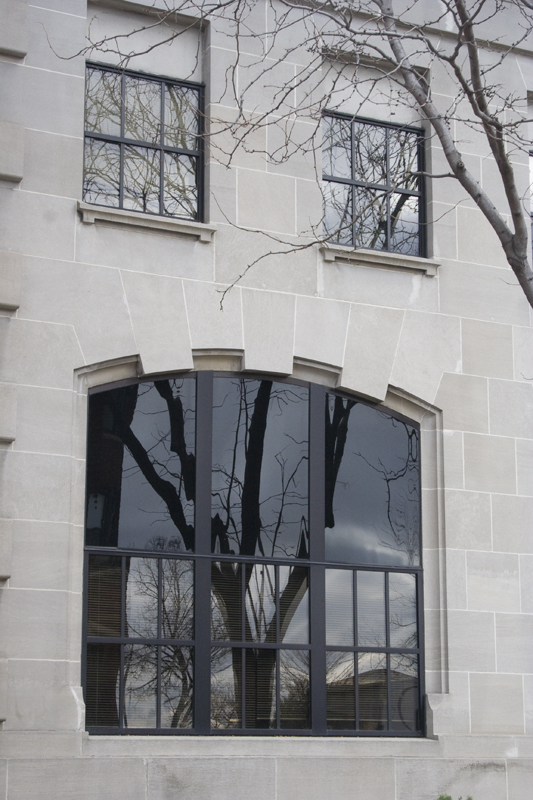
\includegraphics[height=0.6\textheight]{assets/castleface.jpg}
    \caption{\tiny{Credit http://www.flickr.com/photos/slambo\_42}}
  \end{figure}
  \begin{center}
  Susan Potter \small{@SusanPotter} \\
  \tt{CodeMesh} \small{December 2013} \\
  \small{https://github.com/mbbx6spp/funalgebra}
  \end{center}
\end{frame}

%--------------------------------------------------------------------------
% Content
%--------------------------------------------------------------------------

\section{Faces Everywhere}

\begin{frame}{Obvious Face}
  \begin{figure}
    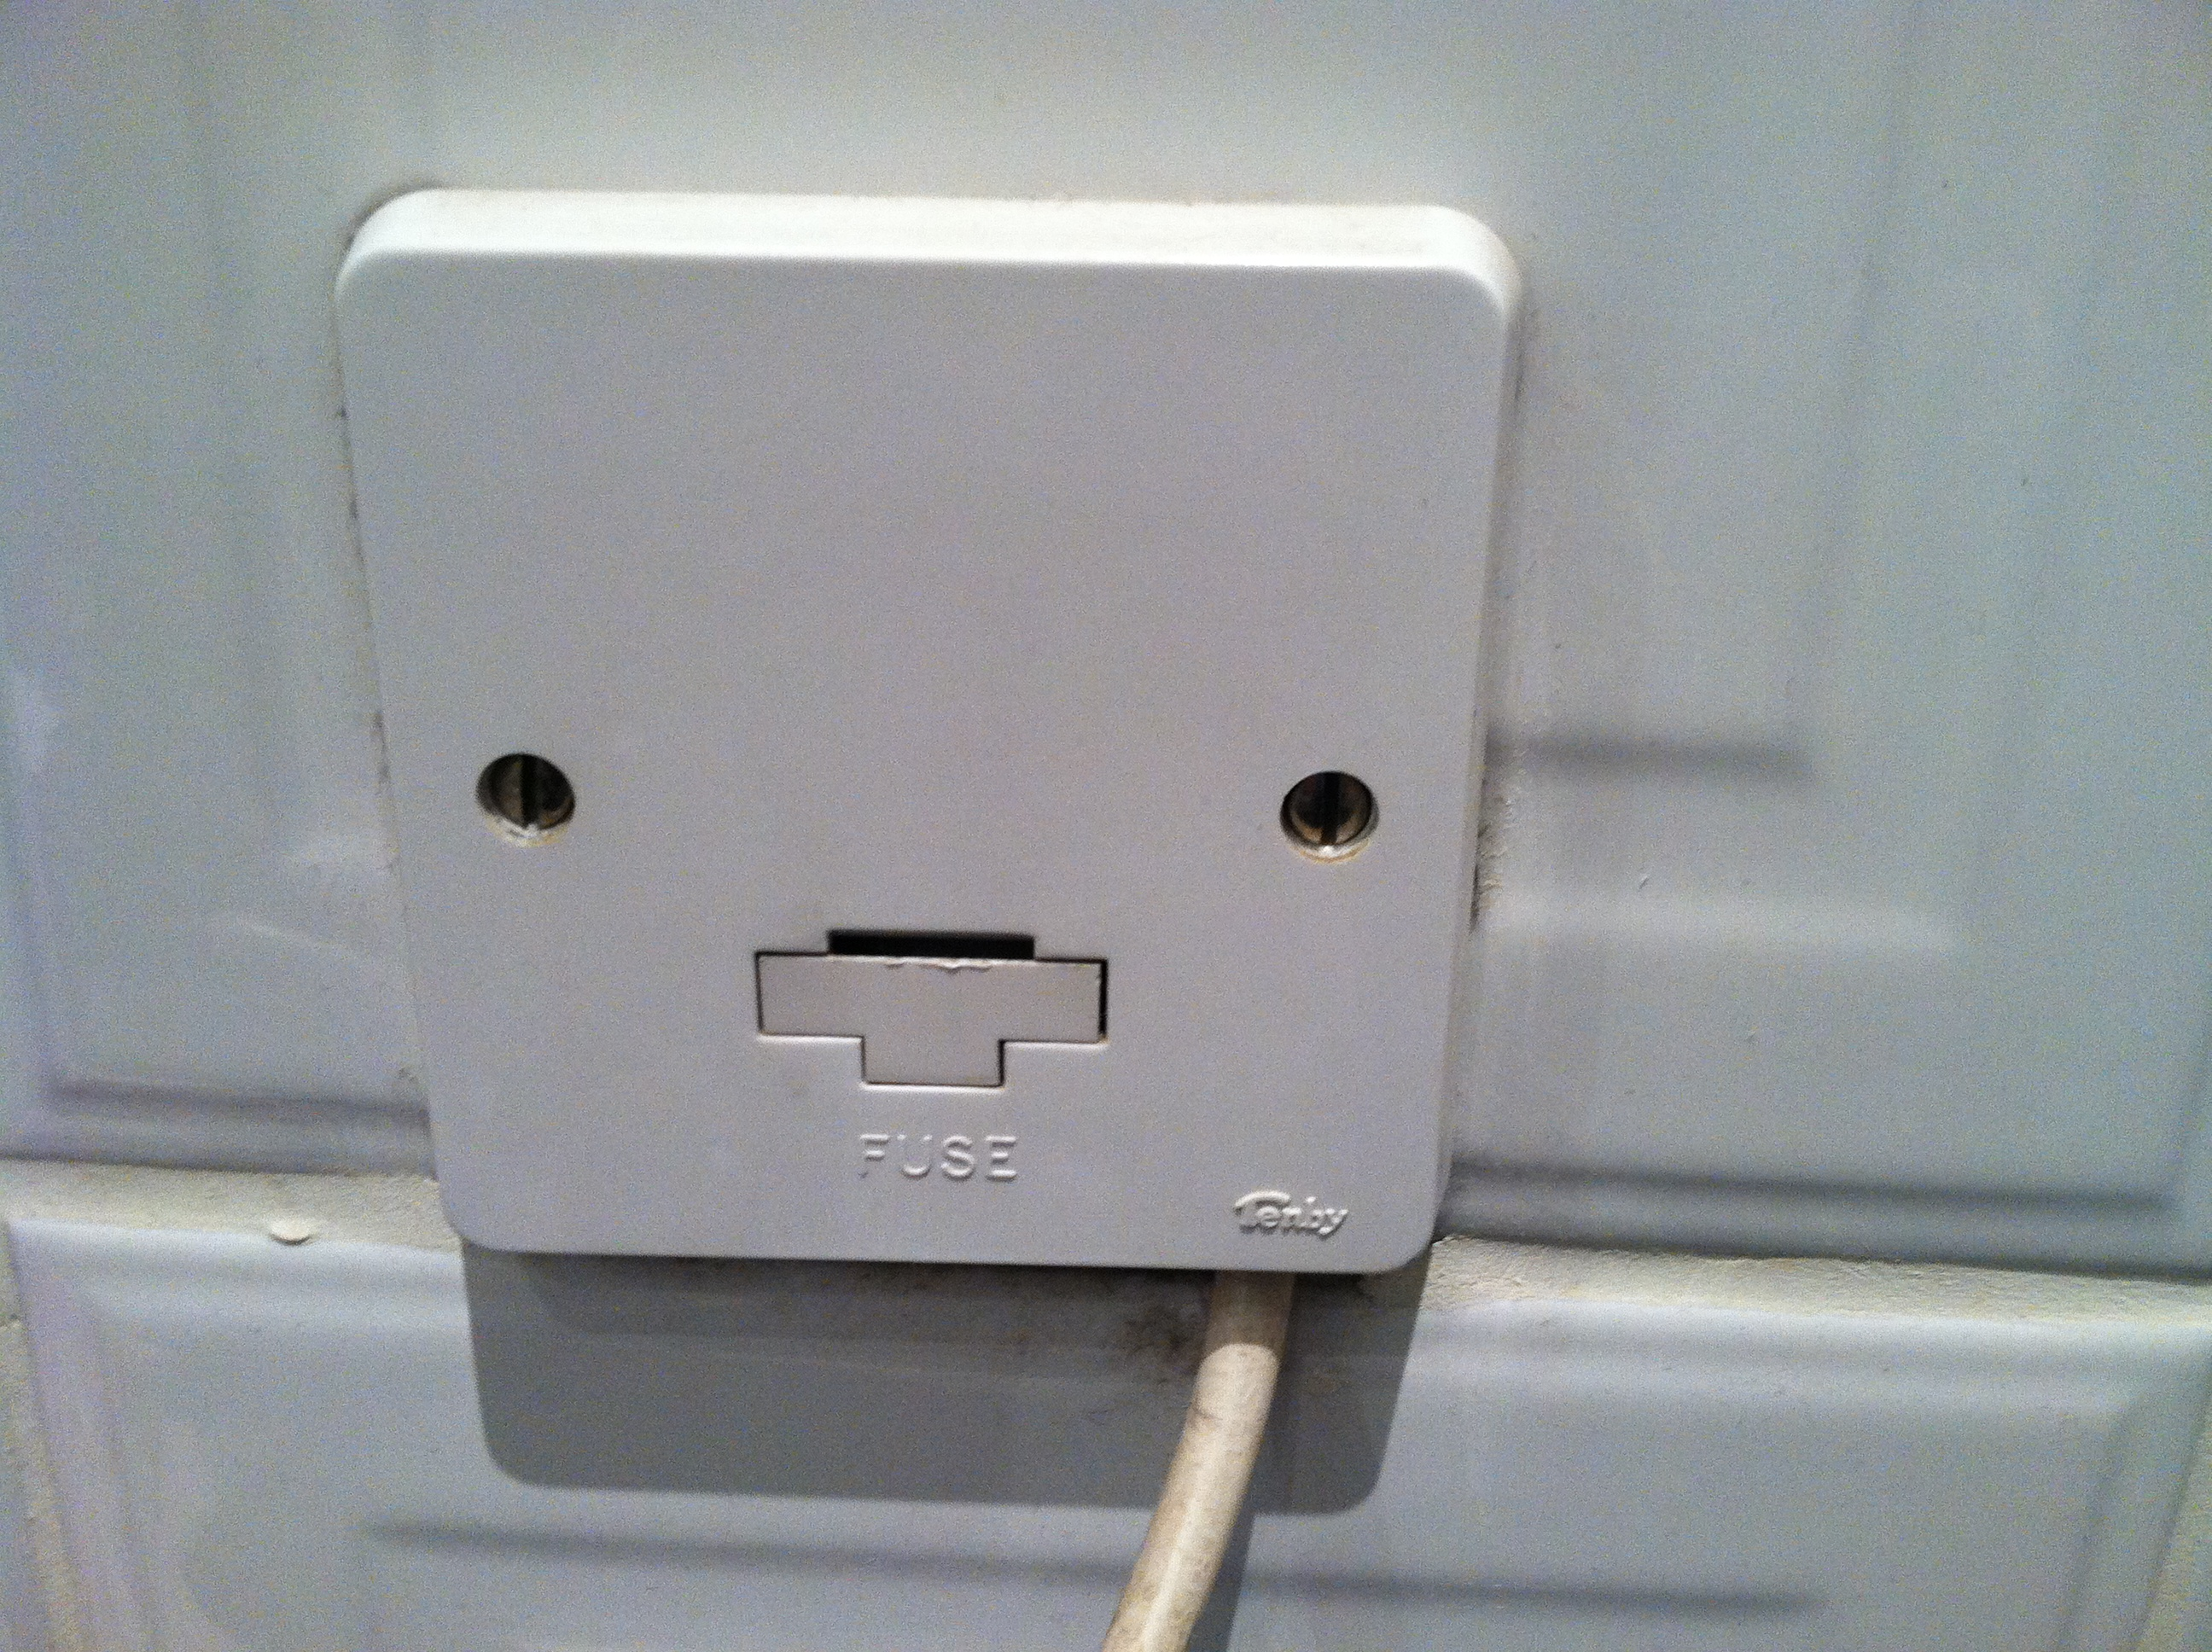
\includegraphics[width=0.9\textwidth]{assets/obviousface.jpg}
  \end{figure}
\end{frame}

\begin{frame}{Less Obvious Face}
  \begin{figure}
    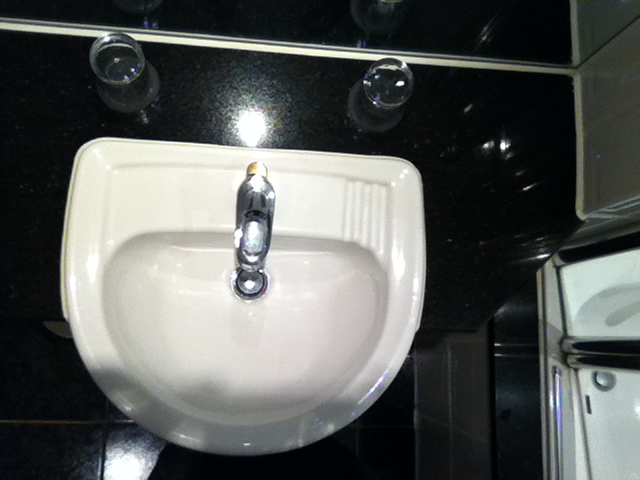
\includegraphics[width=0.9\textwidth]{assets/lessobviousface.jpg}
  \end{figure}
\end{frame}

\begin{frame}{Manufactured Face}
  \begin{figure}
    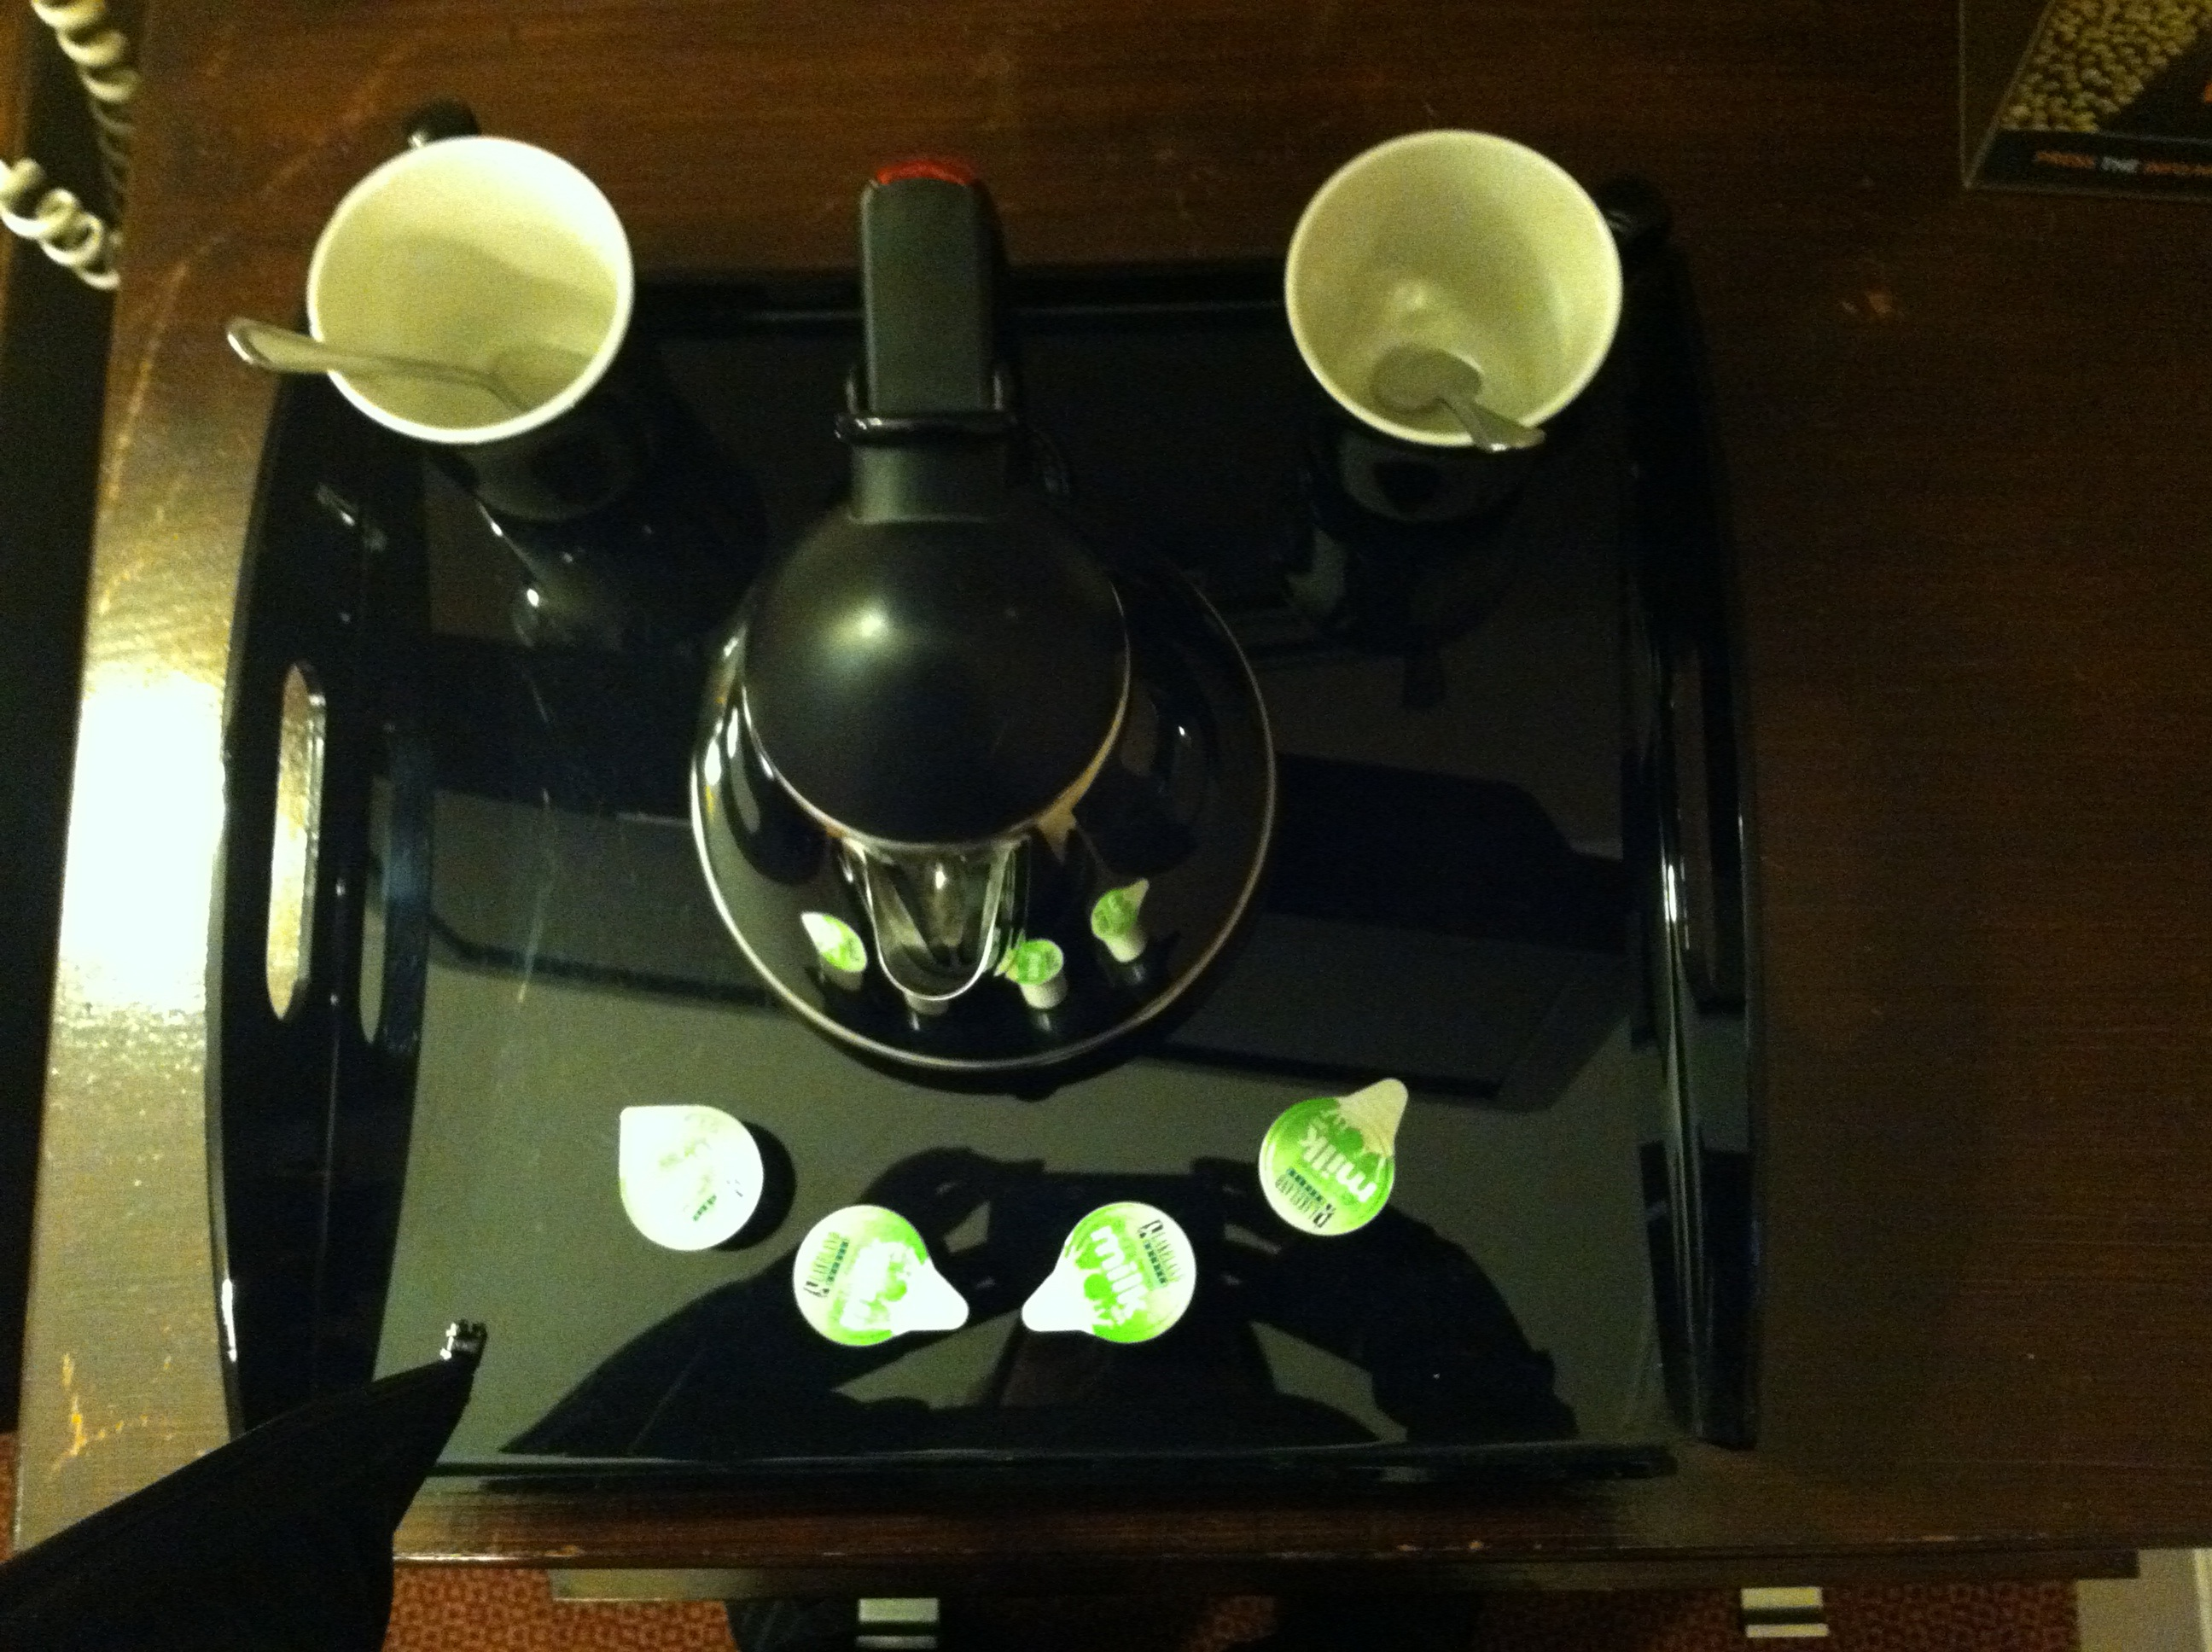
\includegraphics[height=0.8\textheight]{assets/manufacturedface.jpg}
  \end{figure}
\end{frame}

\begin{frame}{Squint Face}
  \begin{figure}
    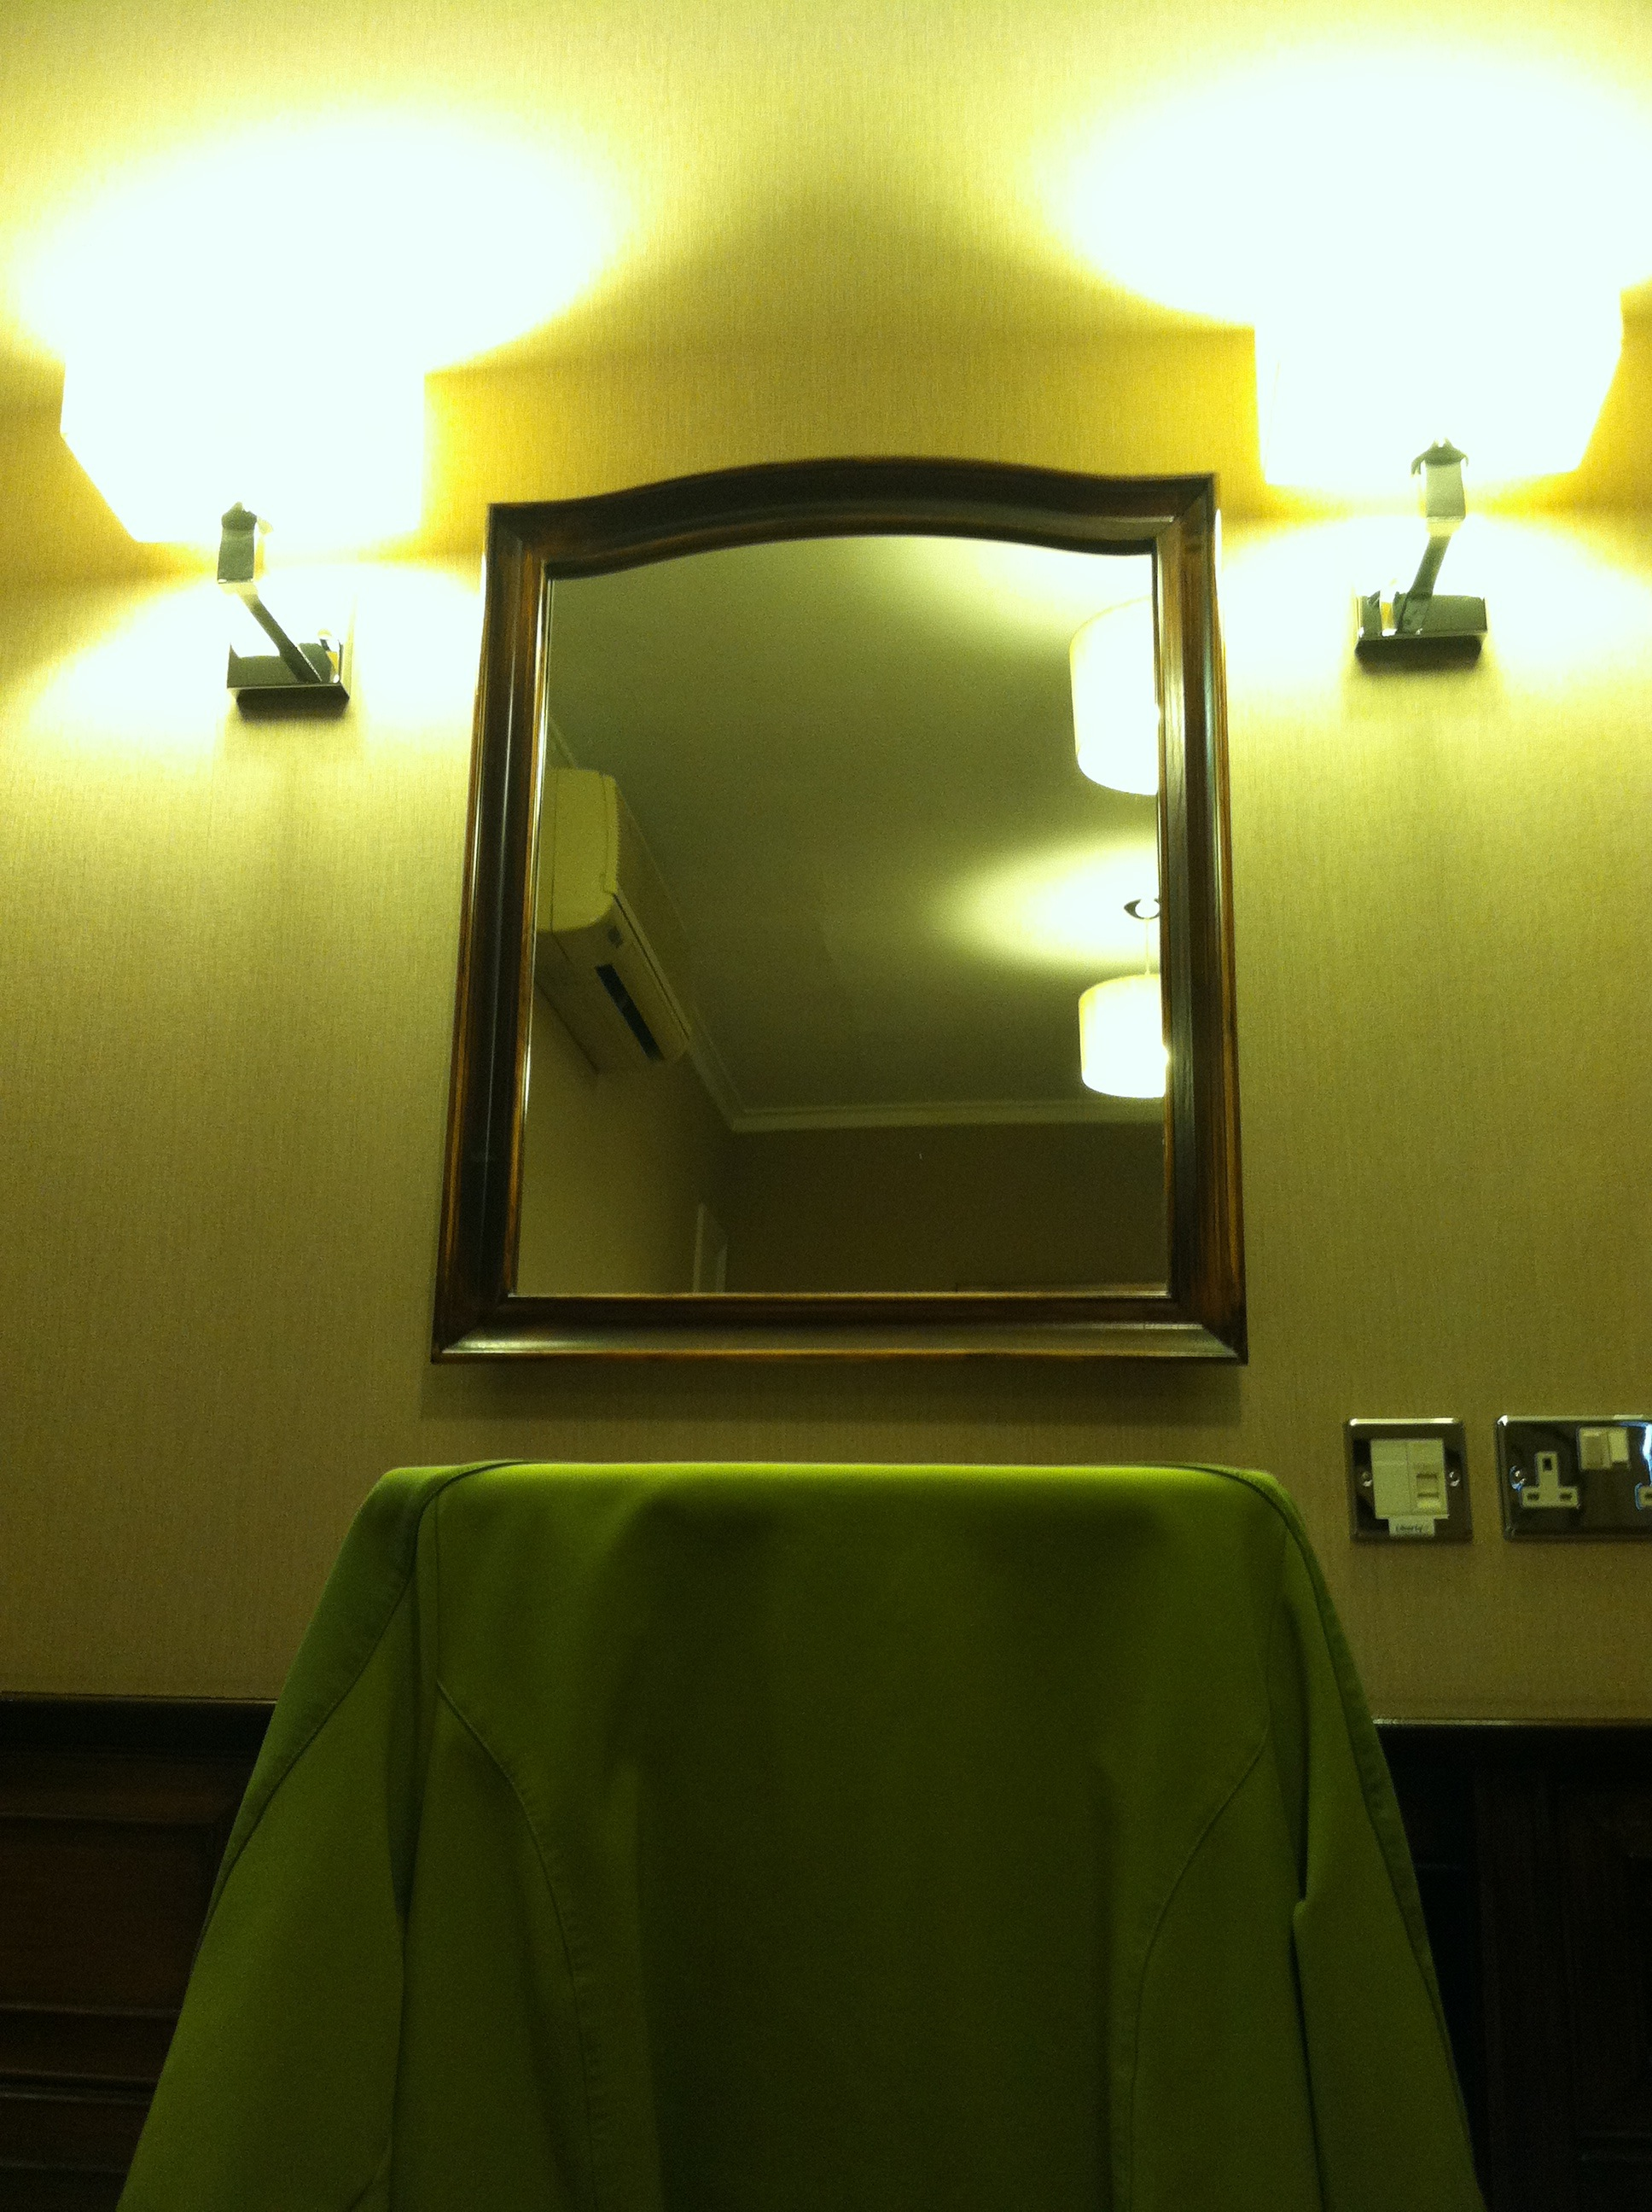
\includegraphics[height=0.8\textheight]{assets/squintface.jpg}
  \end{figure}
\end{frame}

\begin{frame}{Maybe Face}
  \begin{figure}
    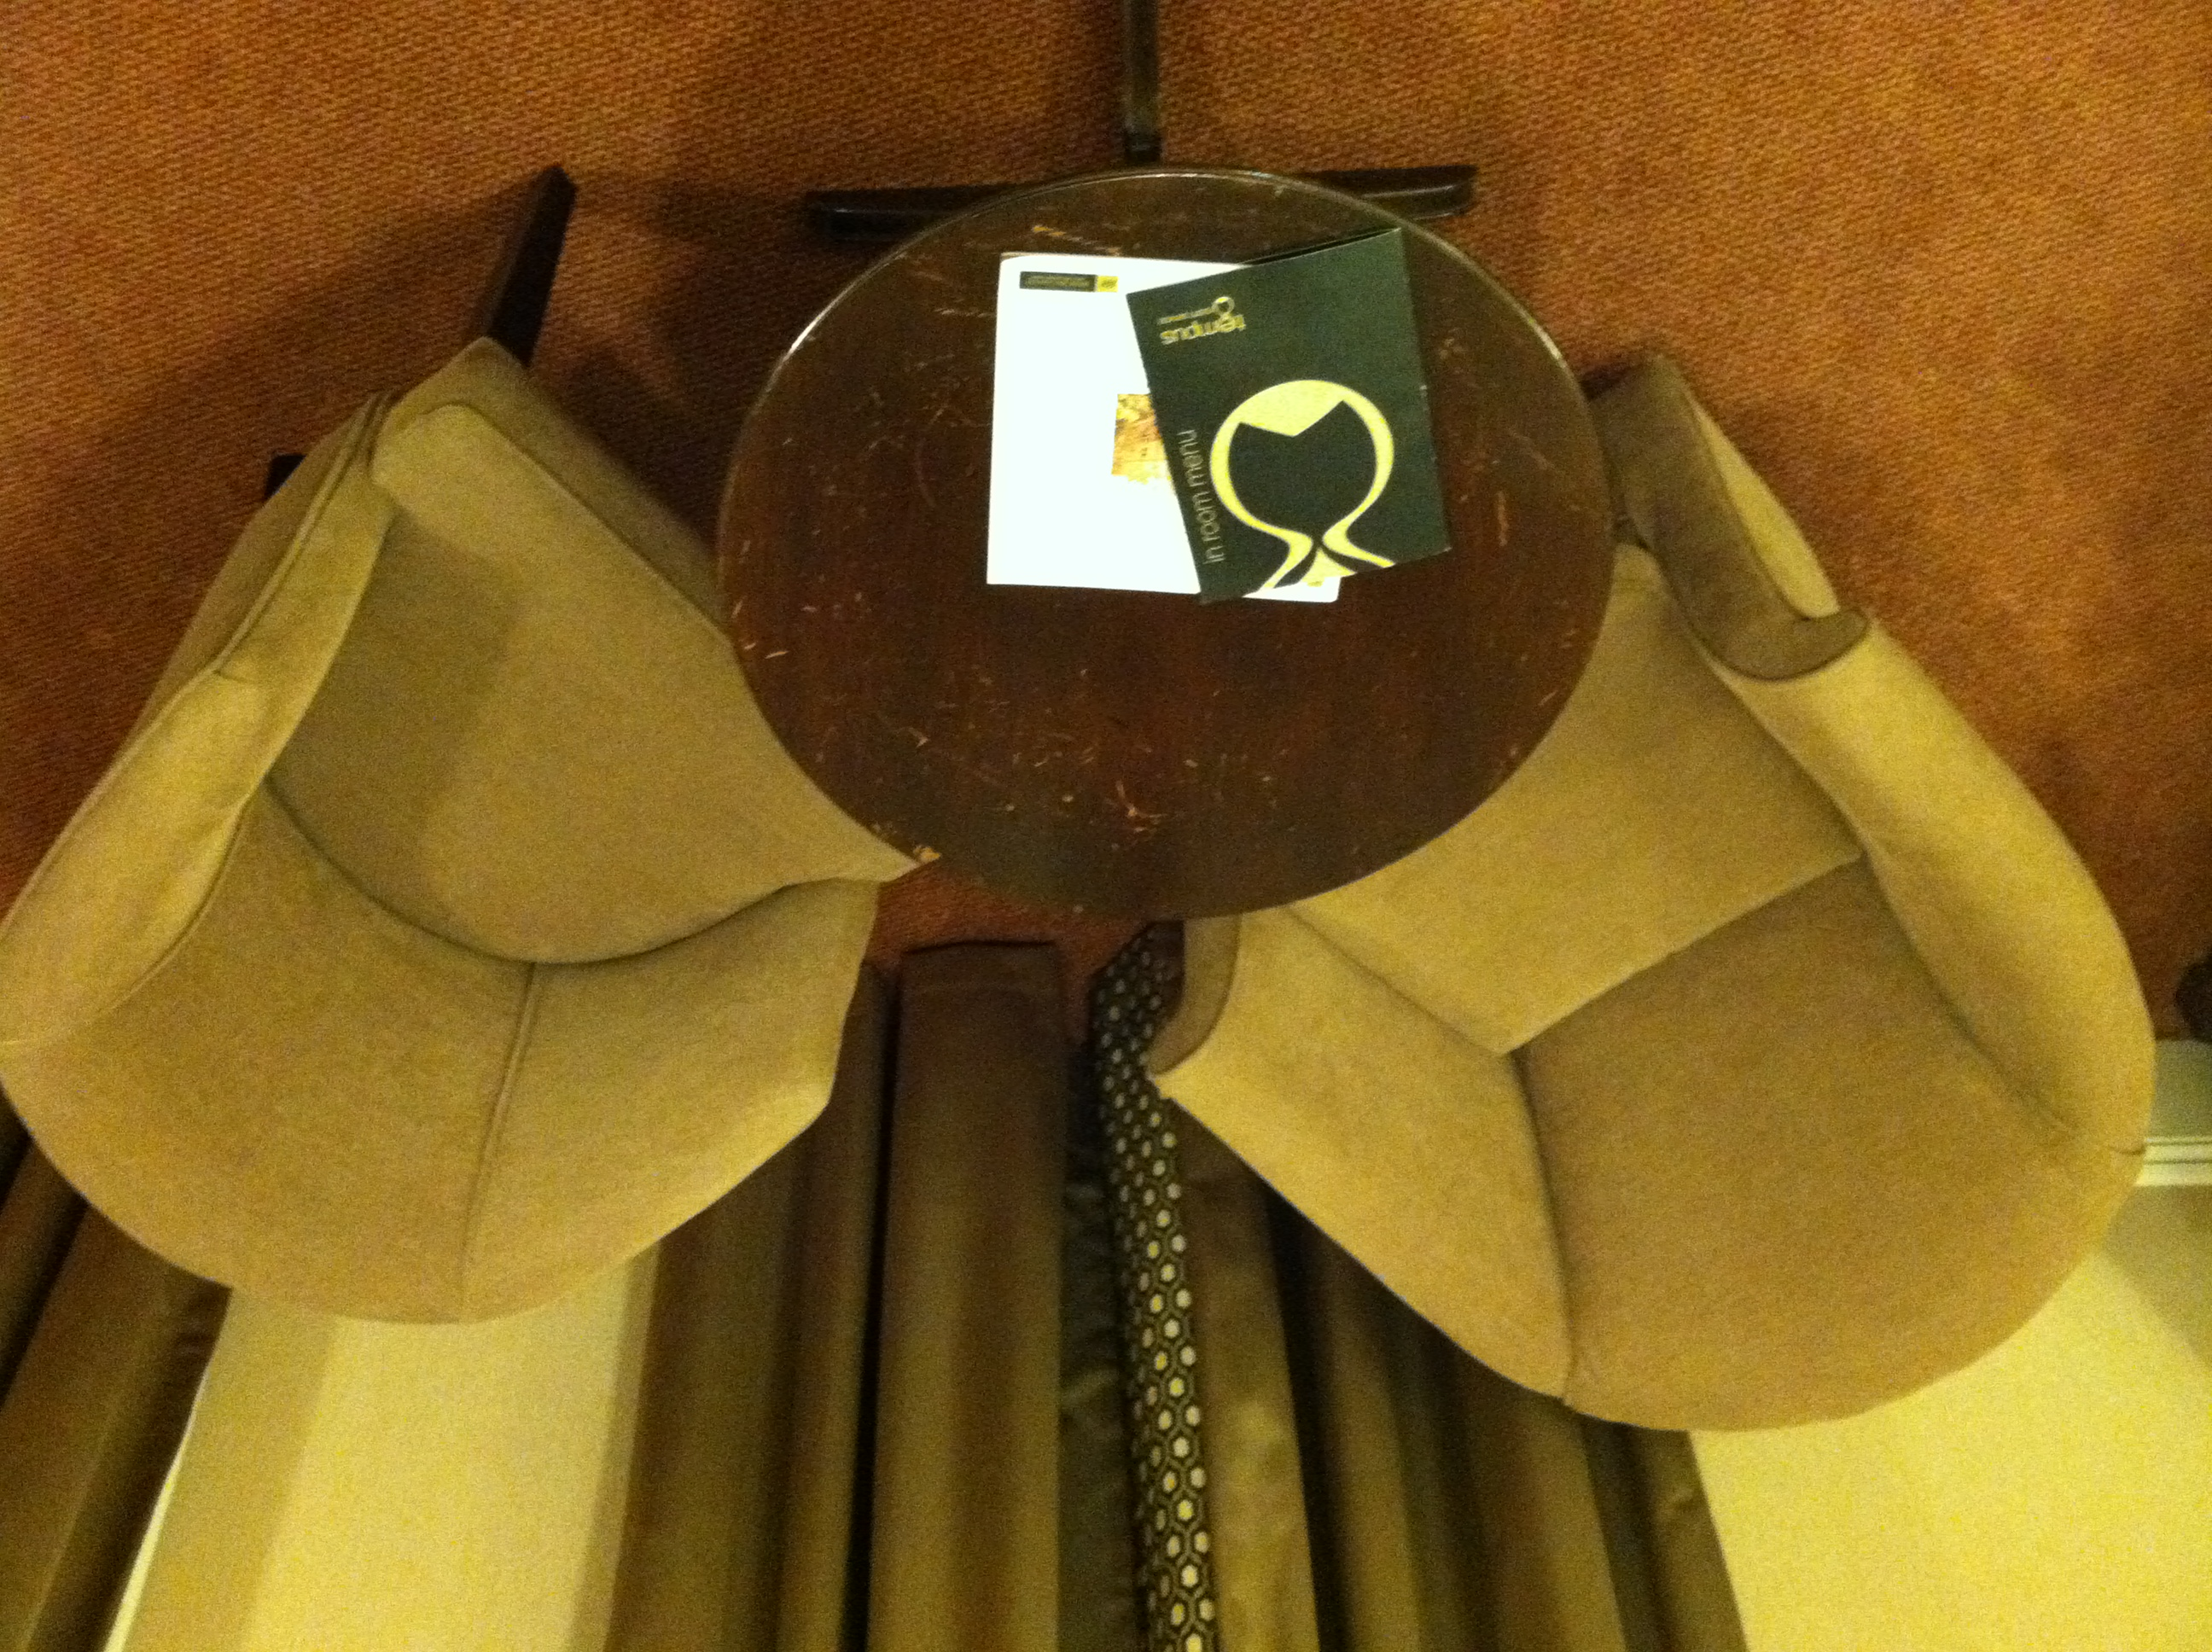
\includegraphics[width=0.8\textwidth]{assets/maybeface.jpg}
  \end{figure}
\end{frame}

\section{Patterns vs Abstractions}

\begin{frame}{OO Patterns vs FP Abstractions}
  \begin{itemize}
    \item \Large{More (Subjective -> Objective)} \newline
    \item \Large{More (Ambiguous -> Precise)} \newline
    \item \Large{"Fluffy" Interfaces -> Generic Functions}
  \end{itemize}
\end{frame}

\begin{frame}{Laying Bricks}
  \begin{figure}
    \centering
    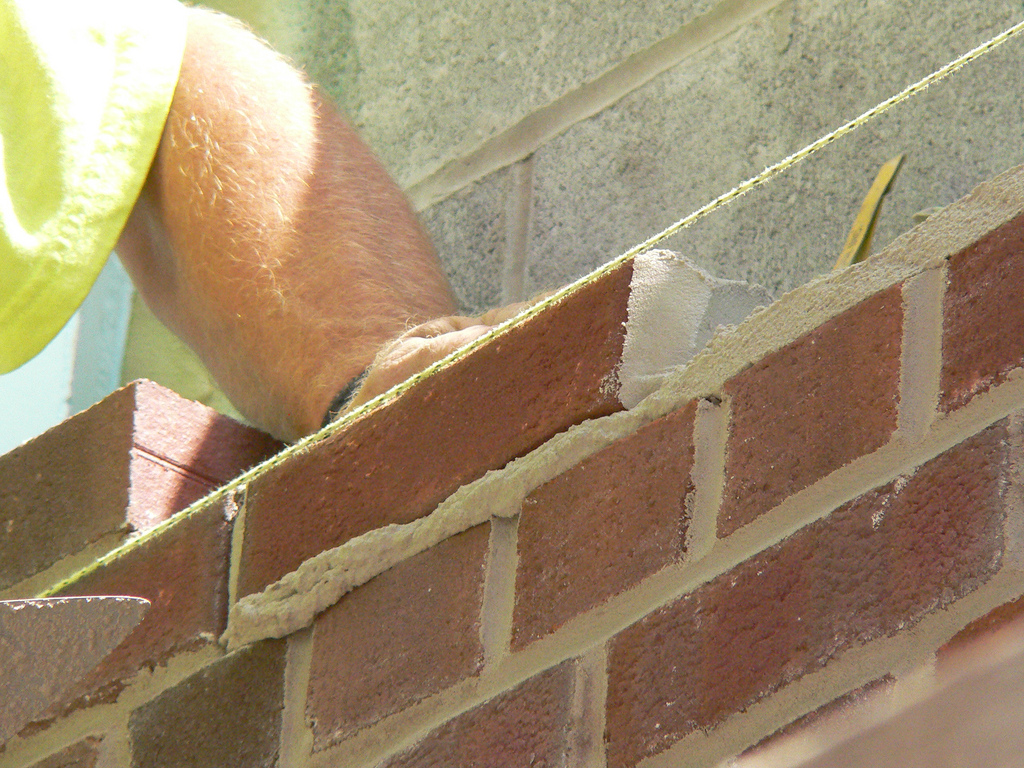
\includegraphics[width=\linewidth]{assets/layingbricks.jpg}
  \end{figure}
\end{frame}

\begin{frame}{Warning}
  \begin{itemize}
    \item \Large{Abstract Algebra -> (Continuous, Infinite)} \newline
    \item \Large{Real World -> usually (Discrete, Finite)}
  \end{itemize}
\end{frame}

\begin{frame}
  \begin{figure}
    \centering
    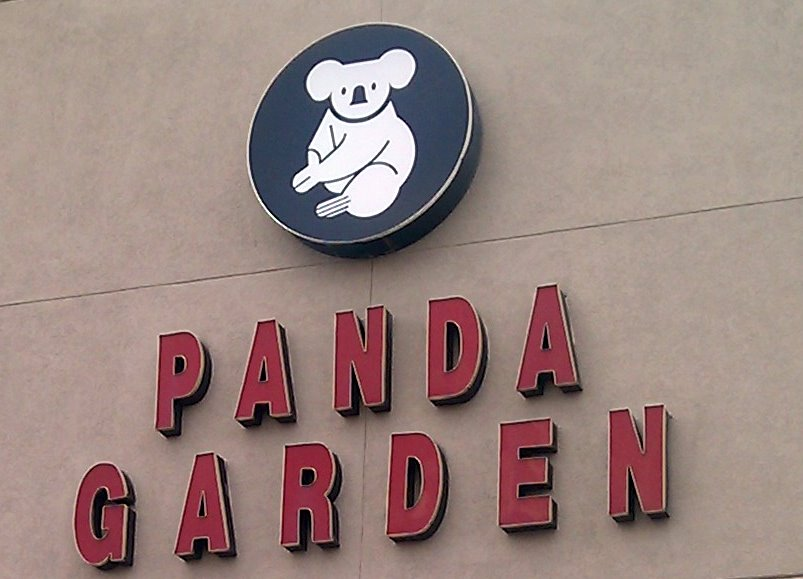
\includegraphics[width=\linewidth]{assets/panda_garden_fail.jpg}
  \end{figure}
\end{frame}

\section{Code}

\begin{frame}[containsverbatim]{Example UNIX Pipe}
\begin{lstlisting}[language=bash]
find . -name "*.rb" \
  | xargs egrep "#.*?TODO:" \
  | wc -l
\end{lstlisting}
  \small{Character-based, through file descriptors}
\end{frame}

\begin{frame}[containsverbatim]{Example Function Composition}
\begin{lstlisting}[language=haskell]
(length . mapToUpper . sanitize) input
\end{lstlisting}
  \small{Value based, through functions}
\end{frame}

\begin{frame}[containsverbatim]{Valuing Values In Real World}
\begin{lstlisting}[language=java]
sealed trait PossiblyMaybe[+A]
final case class Somefink[A](a: A) extends PossiblyMaybe[A]
final case object Nowt extends PossiblyMaybe[Nothing]

object PossiblyMaybeOps {
  def noneDefault[A](pm: PossiblyMaybe[A])(a: A): A = pm match {
    case Somefink(x) => x
    case _ => a
  }
}
\end{lstlisting}
  \small{Note \tt{\_} in second match, caters for \tt{null}s}
\end{frame}

\section{\tt{sbt console}}

\begin{frame}[containsverbatim]{Functor}
\begin{lstlisting}[language=haskell]
class Functor f where
    fmap ∷ (a → b) → f a → f b
\end{lstlisting}
\end{frame}

\begin{frame}[containsverbatim]{Contravariant Functor}
\begin{lstlisting}[language=haskell]
class Contravariant f where
    contramap ∷ (b → a) → f a → f b
\end{lstlisting}
\end{frame}

\begin{frame}[containsverbatim]{Applicative (Functor)}
\begin{lstlisting}[language=haskell]
class (Functor f) => Applicative f where
    pure  :: a -> f a
    (<*>) :: f (a -> b) -> f a -> f b
\end{lstlisting}

\begin{lstlisting}[language=haskell]
-- e.g. using it with Maybe
import Control.Applicative
let incr = (+1)
let mi = Just incr <*> Just 6
-- expect mi to evaluate to Just 7
\end{lstlisting}
\end{frame}

\begin{frame}[containsverbatim]{Bi Functor}
\begin{lstlisting}[language=haskell]
class Bifunctor f where
    bimap ∷ (a → c) → (b → d) → f a b → f c d
\end{lstlisting}
\small{Using over higher kinded types like \tt{Either a b}}
\begin{lstlisting}[language=haskell]
Prelude Data.Bifunctor> :k Either
Either :: * -> * -> *
Prelude Data.Bifunctor> bimap handleFailure handleSuccess eith
\end{lstlisting}
\end{frame}

\begin{frame}[containsverbatim]{Pro Functor}
\begin{lstlisting}[language=haskell]
class Profunctor f where
    dimap ∷ (c → a) → (b → d) → f a b → f c d
\end{lstlisting}
\end{frame}

\begin{frame}{Same Type, Many Interfaces}
  A type defined as a Monad (think: \tt{(>>=)}) can also be used as:
  \begin{itemize}
    \item \Large{A Functor (think: \tt{fmap})} \newline
    \item \Large{An Applicative (think: \tt{<*>, pure})} \newline
    \item \Large{And possibly others} \small{though not necessarily}
  \end{itemize}
\end{frame}

\section{Applications}

\begin{frame}{Known Uses}
\begin{itemize}
  \item \Large{Monoids:} \small{Accumulators are everywhere, almost} \newline
  \item \Large{Functors:} \small{Lots of uses with common and user defined types} \newline
  \item \Large{Monads:} \small{Effects, "Linear Happy Path", and more} \newline
  \item \Large{Applicatives:} \small{"validations", and more} \newline
  \item \Large{More \ldots} \small{e.g. Arrows, Zippers, Lenses, etc.}
\end{itemize}
\end{frame}

\begin{frame}{Thinking Algebraically}
\begin{itemize}
  \item \Large{Properties:} \small{property based testing: quickcheck, scalacheck} \newline
  \item \Large{Data Types:} \small{start closed, extend using "type classes", dependent types, etc when relevant} \newline
  \item \large{Abstractions:} \small{build small building blocks, use motar to build solid walls} \newline
  \item \large{Dist Systems:} \small{using algebraic abstractions, properties to build more useful distributed systems} \newline
\end{itemize}
\end{frame}

\begin{frame}{Royal Fail}
  \begin{figure}
    \centering
    
\includegraphics[width=0.5\textwidth]{assets/royal_fail.jpg}
  \end{figure}
  \tiny{http://www.flickr.com/photos/dadavidov/}
\end{frame}

\begin{frame}{Questions}
  \begin{figure}
    \centering
    
\includegraphics[width=0.5\textwidth]{assets/royal_fail.jpg}
  \end{figure}
  \Large{Questions?}
\end{frame}

\end{document}
